% 3DV 2025 Paper Template; see https://github.com/cvpr-org/author-kit

\documentclass[10pt,twocolumn,letterpaper]{article}

%%%%%%%%% PAPER TYPE  - PLEASE UPDATE FOR FINAL VERSION
% \usepackage{cvpr}              % To produce the CAMERA-READY version
\usepackage{cvpr}   % \usepackage[review]{cvpr}   To produce the REVIEW version
% \usepackage[pagenumbers]{cvpr} % To force page numbers, e.g. for an arXiv version

% Import additional packages in the preamble file, before hyperref
\input{preamble}% Requires XeLaTeX or LuaLaTeX
\usepackage{fontspec}
\usepackage{xspace}

% Load uploaded Caveat-Bold.ttf
\newfontface\SpaceFlowCaveat[
  Path = ./fonts/
]{Caveat-Bold.ttf}

% Exact gradient from #FF66C4 to #FFC259, sampled left-to-right
\definecolor{sfgrad1}{HTML}{FF66C4}
\definecolor{sfgrad2}{HTML}{FF72B7}
\definecolor{sfgrad3}{HTML}{FF7DA9}
\definecolor{sfgrad4}{HTML}{FF899C}
\definecolor{sfgrad5}{HTML}{FF948F}
\definecolor{sfgrad6}{HTML}{FFA081}
\definecolor{sfgrad7}{HTML}{FFAB74}
\definecolor{sfgrad8}{HTML}{FFB766}
\definecolor{sfgrad9}{HTML}{FFC259}

% Robust title logo: no TikZ fading, no clipping
\DeclareRobustCommand{\SpaceFlowLogo}{%
  \texorpdfstring{%
    \raisebox{-0.12ex}{%
      \scalebox{1.55}{%
        {\SpaceFlowCaveat
        \textcolor{sfgrad1}{S}%
        \textcolor{sfgrad2}{p}%
        \textcolor{sfgrad3}{a}%
        \textcolor{sfgrad4}{c}%
        \textcolor{sfgrad5}{e}%
        \textcolor{sfgrad6}{F}%
        \textcolor{sfgrad7}{l}%
        \textcolor{sfgrad8}{o}%
        \textcolor{sfgrad9}{w}}%
      }%
    }%
  }{SpaceFlow}%
}

% Use this in normal paper text
\DeclareRobustCommand{\SpaceFlow}{%
  \texorpdfstring{SpaceFlow}{SpaceFlow}\xspace%
}

\providecommand{\methodname}{}
\renewcommand{\methodname}{\SpaceFlow}
% It is strongly recommended to use hyperref, especially for the review version.
% hyperref with option pagebackref eases the reviewers' job.
% Please disable hyperref *only* if you encounter grave issues, 
% e.g. with the file validation for the camera-ready version.
%
% If you comment hyperref and then uncomment it, you should delete *.aux before re-running LaTeX.
% (Or just hit 'q' on the first LaTeX run, let it finish, and you should be clear).
\definecolor{cvprblue}{rgb}{0.21,0.49,0.74}
\usepackage[pagebackref,breaklinks,colorlinks,citecolor=cvprblue]{hyperref}

% Put this after hyperref is loaded, or in your main .tex after the hyperref block.
\usepackage{mathrsfs}

\usepackage{tikz}
\usepackage{pgfplots}
\usetikzlibrary{arrows.meta,backgrounds}
\pgfplotsset{compat=1.18}

\definecolor{figbg}{HTML}{EEF7F1}
\definecolor{highblue}{HTML}{ADC3F0}
\definecolor{loworange}{HTML}{FFA36F}
\definecolor{deltapurple}{HTML}{8A35FF}

\usepgfplotslibrary{groupplots}

\definecolor{wincol}{HTML}{8BCF9C}
\definecolor{tiecol}{HTML}{D0D0D0}
\definecolor{losscol}{HTML}{E6A09B}

\colorlet{windim}{wincol!35!white}
\colorlet{tiedim}{tiecol!45!white}
\colorlet{lossdim}{losscol!35!white}


%%%%%%%%% PAPER ID  - PLEASE UPDATE
\def\paperID{*****} % *** Enter the Paper ID here
\def\confName{3DV\xspace}
\def\confYear{2025\xspace}

%%%%%%%%% TITLE - PLEASE UPDATE
\title{\mbox{\SpaceFlowLogo}\\ Part-Wise Spatial and Appearence Guidance for 3D Generation}

%alternative title: Locally controllable 3D generation
%%%%%%%%% AUTHORS - PLEASE UPDATE
\author{Neil De La Fuente*\\
ETH Z\"urich\\
{\tt\small nedela@ethz.ch}
\and
Joan Lafuente Baeza*\\
ETH Z\"urich\\
{\tt\small jlafuente@ethz.ch}
\and
Ali Sayfiddinov*\\
ETH Z\"urich\\
{\tt\small msayfiddinov@ethz.ch}
\and
Felicia Scharitzer*\\
ETH Z\"urich\\
{\tt\small fscharitzer@ethz.ch}
}

\begin{document}
\maketitle
\begin{abstract}
Current 3D generators offer limited part-wise control: geometric conditioning is typically applied with a single global strength, while appearance prompts often leak to unintended regions. We present \textbf{\methodname}, a training-free, test-time pipeline for controllable 3D asset generation from text descriptions and editable superquadric primitives. Each primitive serves as a compact proxy for an object part and is assigned a local control level, specifying whether the corresponding region should adhere strictly to the input geometry or adapt to the generative prior. During structure generation, \methodname enforces these constraints locally during the flow process, blending strong guidance in high-control regions with creative completion in low-control regions. For appearance synthesis, the generated structure is segmented and matched to the superquadrics, allowing part-assigned text or image cues to guide the texture of the corresponding regions. Quantitative and qualitative evaluations demonstrate that \methodname preserves specified geometry in high-control regions, enables controlled shape variation, and successfully localizes color, material, and reference-image edits to the intended object parts. 
\end{abstract}    
\begin{figure}[h!]
  \centering
  \includegraphics[width=0.5\textwidth]{figs/teaser.png}
  \caption{\textbf{Part-wise controllable 3D generation using \methodname.} Global prompts are shown at the top, and dashed arrows route reference images to target parts. Orange primitives enforce high spatial (shape-preserving) control; white primitives denote low control. \methodname localizes shape and texture edits to the designated regions.
  \vspace{-5mm}}
  \label{fig:teaser}
\end{figure}

\section{Introduction}
\label{sec:intro}

Modern 3D generative models synthesize increasingly realistic textured assets from text or image prompts~\cite{Xiang_2025_CVPR, hunyuan3d22025tencent, 10.1145/3658146}. However, their control mechanisms remain poorly aligned with practical design and editing workflows. In practice, creators rarely want a single global instruction to dictate an entire asset; rather, they require fine-grained, localized control over both shape and texture. 

For instance, a designer may require one region of an asset to strictly adhere to a target 3D structure while allowing other regions to remain flexible, leveraging the generator's learned prior to plausibly complete or refine the geometry. Similarly, they may want an appearance cue (such as a specific color, material, or reference image) to apply only to a designated component, ensuring no texture leakage occurs elsewhere. This localized intent is difficult to express with existing methods.

% Text prompts are convenient but can be geometrically ambiguous: a phrase such as ``chair with a slat back'' does not specify the exact position, dimensions, or extent of the slats. Image prompts provide stronger visual guidance, but they are difficult to edit directly in 3D and do not naturally expose local control over individual object components. Recent spatial-conditioning methods address this limitation by allowing users to guide generation with explicit 3D geometry, such as coarse primitives or proxy meshes~\cite{fedele2025spacecontrol, 10.1145/3641519.3657425, 10.1145/3641519.3657461}.

% While these methods provide a more direct interface for geometry-aware generation, they typically expose control as a single global trade-off between structural faithfulness and generative realism. Consequently, increasing the control strength preserves the input geometry but over-constrains regions that should be creatively completed, while decreasing it restores geometric plausibility at the expense of losing user-specified structure.

While text and image prompts are convenient, they are often geometrically ambiguous or difficult to edit in 3D. Recent spatial-conditioning methods address this limitation by guiding generation with explicit 3D geometry, such as coarse primitives or proxy meshes~\cite{fedele2025spacecontrol, 10.1145/3641519.3657425, 10.1145/3641519.3657461}. However, these approaches typically enforce control as a single global trade-off: increasing the control strength preserves the input geometry but over-constrains regions that should be creatively completed, while decreasing it restores geometric plausibility at the expense of losing user-specified structure.

% A similar challenge regarding locality arises in appearance control. A global text prompt like ``white sports car with green wheels'' does not explicitly bind the color ``green'' with the wheel geometry. Consequently, appearance conditions may bleed into unrelated parts of the asset or miss the target regions completely. 

% Existing appearance transfer and guidance methods improve texture adaptation by steering pretrained 3D generators or optimizing texture fields~\cite{sayandsarkar_2025_guideflow3d, 10.1145/3588432.3591503, text2mesh, Cohen-Bar_2025_CVPR}, but they are generally formulated as global or whole-object conditioning problems. Enabling controllable asset creation requires a unified interface that specifies not only \textit{what} details the model should generate, but also \textit{where} spatial and appearance controls should apply.

A similar challenge regarding locality arises in appearance control. A flat prompt like ``white sports car with green wheels'' lacks explicit spatial bindings, often causing the green texture to bleed into unrelated parts of the body or fail to cover the wheels entirely. While existing appearance transfer and guidance methods improve texture adaptation~\cite{sayandsarkar_2025_guideflow3d, 10.1145/3588432.3591503, text2mesh, Cohen-Bar_2025_CVPR}, they are generally formulated as global or whole-object conditioning problems. Enabling controllable asset creation requires a unified interface that specifies not only \textit{what} details the model should generate, but also \textit{where} spatial and appearance controls should apply.

We present \textbf{\methodname}, a training-free, test-time pipeline for part-wise controllable 3D asset generation from editable superquadric primitives. Superquadrics provide a compact and intuitive proxy for object structure: they are expressive enough to represent meaningful parts, yet simple enough to manipulate interactively. As illustrated in Fig.~\ref{fig:teaser}, each primitive can be assigned a local control level $\tau$ to govern spatial fidelity, while the same primitive layout serves as a target interface to route local text or image appearance conditions.


% In \methodname, each primitive is assigned a local control level $\tau$, indicating whether the corresponding region should adhere strictly to the input shape or adapt to the generative model's learned geometric prior. The same primitive layout also serves as an interface for part-wise text or image appearance conditions.

We evaluate \methodname on spatial-control and appearance-control tasks covering coarse object sketches, local geometric edits, local color and material conditions, and image-based appearance guidance. We compare our approach against global-control baselines and state-of-the-art appearance transfer methods. Our results show that \methodname preserves the specified geometry in high-control regions, allowing plausible variation in low-control regions and localizing appearance cues to the intended object parts without degrading overall generation quality.
 

In summary, the key contributions of our work are:
\begin{itemize}
    \item We introduce a unified, training-free pipeline for part-wise controllable 3D asset generation that uses superquadrics as a joint interface for shape and appearance.
    \item We propose a localized spatial control formulation for structure generation, enabling different regions of an asset to adopt distinct trade-offs between structural fidelity and generative realism.
    \item We design a part-aware appearance guidance scheme that routes local text or image conditions to target regions, integrated with self-similarity guidance to ensure local coherence and prevent appearance leakage.
\end{itemize}



\section{Related Work}

\noindent Our method builds on recent progress in 3D asset generation by introducing localized spatial and appearance control. We position our work relative to prior state of the art in 3D generation, spatial control, appearance editing, and primitive-based models.


\subsection{3D Asset Generation}
\label{sec:rw_3d_generation}

The field of 3D generation has experienced rapid progress in both output quality and representation flexibility. Early 3D diffusion models operated directly on the original 3D representations, which limited efficiency and possible output types~\cite{nichol2022pointegenerating3dpoint}. Recent approaches have moved generation into compact latent spaces, yielding substantial gains in quality and scalability~\cite{NEURIPS2022_40e56dab,jun2023shapegeneratingconditional3d}. Recent 3D asset generators such as CLAY~\cite{10.1145/3658146}, Hunyuan3D~\cite{hunyuan3d22025tencent}, SAM 3D~\cite{Chen_2026_CVPR}, and TRELLIS~\cite{Xiang_2025_CVPR} further improve fidelity through large-scale training and richer 3D representations. While these models provide strong text, or image, conditioned generation, they are conditioned globally and do not support local, part-wise control.

% While these models provide strong text or image conditioned generation, they do not offer explicit part-wise control over where geometric and appearance conditions should apply.


\subsection{Spatially Controllable 3D Generation} 
\label{sec:rw_spatial_control}

Spatially controllable generation shifts conditioning from ambiguous text or image prompts to explicit 3D inputs, such as voxels, primitives, proxy shapes, or meshes. Existing methods can be grouped into training-based and test-time approaches. Training-based methods fine-tune generative models to accept geometric conditions~\cite{NEURIPS2022_40e56dab, 10.1145/3641519.3657461}. These approaches can provide direct spatial control, but require additional training costs and are often tied to the conditioning format and data distribution used during training. 

Test-time methods inject spatial conditions during inference, either via optimization or latent projection. Optimization-based approaches project 3D constraints into rendered views or optimize an explicit 3D representation under geometric guidance~\cite{Metzer_2023_CVPR,10.1145/3641519.3657425}. SpaceControl~\cite{fedele2025spacecontrol} is closest to our work: it injects a user-specified 3D geometry into the latent space of a pretrained 3D generator and exposes a control strength that trades geometric fidelity for generative realism. However, this trade-off is applied globally. A single control strength cannot express common design intent where some regions should remain faithful to the input geometric control while others should be completed or reshaped by the generative prior. 

\subsection{Appearance and Texture Control for 3D Assets} 
\label{sec:rw_appearance_control}

Appearance control has been widely explored across various 3D formats. For meshes, existing methods generate or edit textures using text prompts, image priors, or learned neural fields~\cite{text2mesh, 10.1145/3588432.3591503, perla2024easitex, Cohen-Bar_2025_CVPR}, while related work extends these stylization techniques to implicit radiance fields and Gaussian splats~\cite{liu2023stylerf, liu2023stylegaussian, 10.1007/978-3-031-85187-2_15}. Although these approaches can produce high-quality appearance edits, they are typically tied to a specific output representation or operate on an existing asset rather than controlling the appearance stage of a generative 3D pipeline.

GuideFlow3D~\cite{sayandsarkar_2025_guideflow3d} is closest to our appearance-control setting, as it performs training-free guidance of a pretrained rectified-flow model and introduces a self-similarity loss for robust appearance transfer. However, GuideFlow3D is designed for global style transfer, applying an overall appearance specification to the entire asset.  In contrast, our approach enables part-wise appearance control. Instead of relying on global prompts or reference images that indirectly affect the whole object, we introduce a direct interface that routes specific appearance cues to designated object parts, preventing texture leakage.


\subsection{Primitive-Based and Part-Aware Editing}
\label{sec:rw_part_primitive_editing}

A complementary line of work aims to make 3D assets editable by exposing an intermediate structure in the form of primitives, parts, graphs, or programs. 

Primitive-abstraction methods approximate shapes with compact geometric elements, ranging from volumetric primitives to superquadrics and learned neural primitives~\cite{abstractionTulsiani17,Paschalidou2019CVPR,Paschalidou2021CVPR}. These decompositions provide interpretable manipulation handles, but are typically designed for abstraction or reconstruction and remain tied to the chosen primitive family or learned parser.


Part-aware generative models make object structure explicit during generation. StructureNet~\cite{MoGuerreroEtAl:StructureNet:SiggraphAsia:2019} and ShapeAssembly~\cite{jones2020shapeAssembly} represent shapes through hierarchical part graphs or executable programs over cuboid proxies. Later neural approaches build part-level manipulation into implicit shapes, local radiance fields, or diffusion-based point and latent representations, enabling operations such as part transformation, recombination, completion, and mixing~\cite{hertz2022spaghetti,Tertikas2023CVPR,koo2023salad,nakayama2023difffacto}.

Recent methods extend this idea toward more realistic and higher-fidelity asset generation: PartGen~\cite{Chen2025PartGen} reconstructs objects as meaningful editable parts, while CompoSE~\cite{slim2026composecompositionalsynthesisediting}, the closest prior in this line, uses coarse geometric primitives such as bounding boxes as part controls to synthesize part-separated objects for localized editing.

These methods demonstrate the value of explicit part structure, but typically require the generated asset itself to be represented, generated, or reconstructed as a set of parts.

\section{Method}

\begin{figure*}[t!]
  \centering
  \includegraphics[width=0.95\textwidth]{figs/mainfig_3.pdf}
  \caption{\textbf{\methodname pipeline.} Given editable superquadric controls with per-primitive spatial conditioning strengths $\tau_i$, SpaceFlow encodes the high-control regions and injects them into the TRELLIS sparse-structure flow process over a controlled time interval. The resulting structure is then passed to a texture flow model, where optional per-part text or image conditions are routed through PartField segments and refined with self-similarity guidance, producing a 3D asset with localized spatial and appearance control.
  \vspace{-4mm}}
  \label{fig:overview}
\end{figure*}

We present our method for part-wise spatial and appearance guidance for 3D Generation, detailing our superquadric primitives, pipeline architecture, and spatial and appearance control formulations.

\subsection{Problem Formulation}
% Given a text prompt $p$, a user-edited set of deformable superquadric primitives $\mathcal{S}=\{S_i\}_{i=1}^{N}$, per-primitive control levels $\boldsymbol{\tau}=\{\tau_i\}_{i=1}^{N}$, and optional appearance cues $\mathcal{A}=\{a_i\}$, our goal is to generate a textured 3D asset $X=(G,T)$ whose geometry and appearance obey the user constraints locally. Each primitive $S_i$ defines a spatial region of intent, while $\tau_i$ controls how strongly the generated geometry should follow that region. High values of $\tau_i$ enforce close adherence to the scaffold; lower values allow the generative prior to reinterpret or complete the region. When an appearance cue $a_i$ is provided, it should affect only the corresponding primitive region.
Given a text prompt $p$, a user-edited set of deformable superquadric primitives $\mathcal{S}=\{S_i\}_{i=1}^{N}$, per-primitive control levels $\boldsymbol{\tau}=\{\tau_i\}_{i=1}^{N}$ with $\tau_i \in \{\tau_{\text{low}}, \tau_{\text{high}}\}$, and optional appearance cues $\mathcal{A}=\{a_i\}$, our goal is to generate a textured 3D asset $X=(G,T)$ whose geometry and appearance obey the user controls locally. The conditioning strengths $\tau_{\text{low}}$ and $\tau_{\text{high}}$ are user-defined values within the range $[0, 12]$ satisfying $\tau_{\text{low}} < \tau_{\text{high}}$. Each primitive $S_i$ defines a spatial region of intent, while its control strength $\tau_i$ determines the local trade-off between shape fidelity and generative completion. Primitives assigned to the high-control strength $\tau_{\text{high}}$ enforce strict adherence to the input geometry, whereas primitives assigned to the low-control strength $\tau_{\text{low}}$ allow the generative prior to reinterpret or complete the region. When an appearance cue $a_i$ is provided, it must affect only the corresponding primitive region $i$.

% Unlike part-based generators, we do not require the final asset to be represented as a set of generated parts. The primitive scaffold is used only as localized guidance for a pretrained 3D generator: constrained regions should respect the user input, while unconstrained regions remain free to be completed plausibly.

\subsection{Superquadric Primitives}
\label{sec:superquadric_primitives}
Superquadrics are compact primitives that span ellipsoidal, cylindrical, rounded-box, and box-like shapes~\cite{1673799}. Each control primitive is parameterized as $S_i(\mathbf{R}_i,\mathbf{t}_i,\mathbf{s}_i,\boldsymbol{\epsilon}_i,\boldsymbol{\delta}_i)$, where $(\mathbf{R}_i,\mathbf{t}_i)$ is its pose (rotation matrix and translation vector), $\mathbf{s}_i = (s_{x,i}, s_{y,i}, s_{z,i})^\top$ its scale, $\boldsymbol{\epsilon}_i = (\epsilon_{1,i}, \epsilon_{2,i})^\top$ its shape exponents, and $\boldsymbol{\delta}_i$ its deformation parameters.
For a 3D point $\mathbf{x}$, let $\mathbf{u} = (u_x, u_y, u_z)^\top = \mathbf{R}_i^\top(\mathbf{x}-\mathbf{t}_i)$ be its coordinates in the primitive's local frame. Ignoring deformations, the superquadric volume is defined by the implicit inequality $F_i(\mathbf{x})\leq 1$, where the inside-outside function $F_i(\mathbf{x})$ is given by:
\vspace{-3mm}
\begin{equation}
F_i(\mathbf{x}) = \left( \left|\frac{u_x}{s_{x,i}}\right|^{2/\epsilon_{2,i}} + \left|\frac{u_y}{s_{y,i}}\right|^{2/\epsilon_{2,i}} \right)^{\epsilon_{2,i}/\epsilon_{1,i}} + \left|\frac{u_z}{s_{z,i}}\right|^{2/\epsilon_{1,i}} .
\label{eq:superquadric_implicit}
\end{equation}
In our scaffold, the deformation parameter $\boldsymbol{\delta}_i$ adds bending and tapering degrees of freedom, making the primitives more expressive than raw superquadrics. We use these deformable superquadrics as editable spatial control regions, not as the final output representation.


% \subsection{Two-Stage 3D Generation Backbone}
% \label{sec:trellis_backbone}

\subsection{Architecture Overview}

% Our method builds upon TRELLIS, which is a pretrained 3D generation backbone~\cite{Xiang_2025_CVPR}. TRELLIS represents an asset with a structured latent representation, SLAT, consisting of a sparse set of active voxels and local latent features attached to those voxels. The representation captures both geometry and appearance and can be decoded into meshes, radiance fields, or Gaussian splats.
Our method is built upon TRELLIS~\cite{Xiang_2025_CVPR}, a pretrained 3D generation backbone. TRELLIS represents 3D assets using a structured latent representation (SLAT), which consists of a sparse set of active voxels and local latent features attached to those voxels. This representation jointly captures geometry and appearance, and can be decoded into multiple formats including meshes, neural radiance fields, or Gaussian splats.

%TRELLIS generates SLAT in two stages. A first rectified-flow transformer generates the sparse voxel structure, which determines the coarse 3D support of the object. A second rectified-flow transformer then generates the local latent features on the active voxels, after which a decoder produces the final textured asset. 
TRELLIS generates this representation in two stages. First, a rectified-flow transformer generates the sparse voxel structure that defines the coarse 3D support of the object. Second, a subsequent rectified-flow transformer generates the local latent features on the active voxels, after which the VAE decoder produces the final textured asset. 

%This factorization makes TRELLIS well suited to our setting: we guide the structure stage with spatial conditions from user-edited primitives (see Section~\ref{sec:spatial_local_control}), and guide the latent stage with localized per-primitive appearance cues (see Section~\ref{sec:appearance_local_control}).

% An overview of our proposed pipeline is illustrated in Fig.~\ref{fig:overview}. The system takes as input a set of editable superquadric control shapes with associated spatial conditioning strengths $\tau_i$, along with optional text prompts or reference images for texture control. The spatial control inputs are processed via the Structure Flow Model (Section~\ref{sec:spatial_local_control}) to synthesize the coarse 3D voxel structure. The resulting structure is then decoded and passed to the Texture Flow Model (Section~\ref{sec:appearance_local_control}), where localized per-part text or image conditions are routed to specific sections of the asset via a segmented PartField representation and synthesized using self-similarity guidance.
This decoupled architecture is uniquely suited to our localized control setting. As outlined in Fig.~\ref{fig:overview}, the user-edited superquadrics and their spatial conditioning strengths $\tau_i$ guide the Structure Flow Model (Section~\ref{sec:spatial_local_control}) to generate the coarse 3D voxel structure. This structure is then decoded and passed to the Texture Flow Model (Section~\ref{sec:appearance_local_control}), where localized text prompts or reference images are routed to target sections of the asset via a segmented PartField representation and generated under self-similarity guidance.

\subsection{Local Spatial Control for Structure Generation}
\label{sec:spatial_local_control}
%describe the weighted avg,repaint, injection... @joan

To implement local spatial control during structure generation, we partition the user-defined superquadrics $\mathcal{S}$ into high-control ($\mathcal{S}_{\text{high}}$) and low-control ($\mathcal{S}_{\text{low}}$) subsets based on their individual conditioning strengths $\tau_i$. We also define noise thresholds $\tau_{\text{low}}$ and $\tau_{\text{high}}$ in the flow model's trajectory, which govern the timesteps over which these spatial controls are active. 

First, we render the complete set $\mathcal{S}$ and the high-control subset $\mathcal{S}_{\text{high}}$ independently. Both renders are encoded into the structure space using the VAE of TRELLIS to obtain the clean latents $\mathbf{z}_0^{\text{all}}$ and $\mathbf{z}_0^{\text{high}}$. Additionally, we define a binary spatial mask $\mathbf{M}_{\text{low}}$ by generating a bounding box around $\mathcal{S}_{\text{low}}$ with a $7\%$ spatial padding, which is then downsampled to the latent dimensions ($16 \times 16 \times 16$) using a $4 \times 4 \times 4$ 3D max pooling operation.

Following SpaceControl, we initialize the process by perturbing $\mathbf{z}_0^{\text{all}}$ with noise corresponding to the timestep $\tau_{\text{low}}$, yielding the initial noisy latent $\mathbf{z}_{\tau_{\text{low}}}^{\text{all}}$. We then begin the denoising process from this state to establish the coarse layout of the low-control components.

To ensure that the structural details of the high-control regions are preserved in the output, we inject the clean high-control latent $\mathbf{z}_0^{\text{high}}$ at each denoising step $t$. Using the low-control mask $\mathbf{M}_{\text{low}}$, we compute a spatially masked weighted average to obtain the updated latent $\mathbf{z}'_t$:
\begin{equation}
\mathbf{z}'_t = (1 - \mathbf{M}_{\text{low}}) \odot \left( \alpha \mathbf{z}_0^{\text{high}} + (1 - \alpha) \mathbf{z}_t \right) + \mathbf{M}_{\text{low}} \odot \mathbf{z}_t
\label{eq:high_control_injection}
\end{equation}
where $\mathbf{z}_t$ is the model's denoised prediction, $\odot$ denotes the element-wise product, and the blending weight is set to $\alpha = 0.18$. This hyperparameter was chosen experimentally but can be adjusted depending on the specific asset being generated.

To improve the transition boundaries between the high, and low, control regions, we apply a resampling strategy following RePaint~\cite{lugmayr2022repaint}. Following the noise scheduler, we perform $N$ iterations of a resampling loop. In each iteration, we first perturb the blended sample from $t_{i-1}$ back to step $t_i$. We then denoise the sample back to $t_{i-1}$ using a single solver step and re-apply the blending formulation in Eq.~\eqref{eq:high_control_injection}. This iterative blending is performed for the steps between $\tau_{\text{low}}$ and $\tau_{\text{high}}$, corresponding to the \textit{Conditioned Flow} phase shown in Fig.~\ref{fig:overview}.

% To improve the transition boundaries between the high- and low-control regions, we apply a resampling strategy inspired by RePaint~\cite{repaint}. We define the timestep difference $\Delta t = t_i - t_{i-1}$ following the noise scheduler and perform $N$ iterations of a resampling loop. In each iteration, we first perturb the blended sample back to step $t_i$. 

% Following the linear interpolation framework of flow matching, this local re-noising step over the interval $\Delta t$ is formulated as:
% \begin{equation}
% \mathbf{z}_{t_i} = (1 - \Delta t) \mathbf{z}'_{t_{i-1}} + \Delta t \mathbf{\epsilon}, \quad \mathbf{\epsilon} \sim \mathcal{N}(\mathbf{0}, \mathbf{I})
% \label{eq:repaint_renoising}
% \end{equation}
%where $\mathbf{z}'_{t_{i-1}}$ acts as the local clean reference. 



\subsection{Matching Generated Parts to Superquadrics}
\label{sec:part_matching}
To route appearance cues to the correct regions, we establish a correspondence between the generated structure and the input primitives $\mathcal{S}$. A direct geometric assignment is unreliable: low-control regions are reshaped by the generative prior and no longer align with their primitives, so nearest-primitive labelling yields fragmented, semantically inconsistent regions. We therefore match parts in a learned part-aware feature space.

Given the generated structure mesh, we extract a PartField~\cite{liu2025partfield} triplane feature field $\mathcal{P}$, which encodes part-level semantics learned across large 3D collections. For each active structure voxel $\mathbf{v}_j$ on the $64^3$ grid, we sample $\mathcal{P}$ at its normalized position by interpolating the three axis-aligned planes and summing them, yielding a $448$-dimensional descriptor $\mathbf{f}_j$. We $\ell_2$-normalize these descriptors and cluster them with $K$-means into $K{=}10$ semantic parts, assigning each voxel a part label $\ell_j$.

We then assign each part-cluster to a single primitive. Each $S_i$ is voxelized to its set of surface cells $\mathcal{B}_i$. For each cluster $C_k$ we take the voxel $\mathbf{c}_k$ closest to the cluster's spatial mean as its representative, and assign the whole cluster to the nearest primitive:
\vspace{-2mm}
\begin{equation}
a(k) = \arg\min_{i} \min_{\mathbf{b}\in\mathcal{B}_i} \lVert \mathbf{c}_k - \mathbf{b}\rVert_2 .
\label{eq:cluster_assignment}
\end{equation}
Every voxel inherits the primitive label $a(\ell_j)$ of its cluster. Operating at the cluster level rather than per voxel makes the assignment robust: an entire semantic part is routed to one primitive even where the generated geometry has drifted from the scaffold. The resulting labels are downsampled to the $32^3$ latent grid to form a dense routing volume $\mathbf{R}$, whose occupied cells store the index of the assigned primitive ($0$ denotes the global fallback).

Because routing is performed on the coarse $32^3$ grid, thin or small primitives (\eg wheels) may collapse to too few cells to carry their local cue. We therefore (i) fall back to a purely geometric per-voxel nearest-primitive assignment whenever cluster-based routing fails to cover a primitive holding an active local cue, and (ii) adaptively grow any under-covered primitive up to a minimum cell count by dilation, never overwriting cells already claimed by another primitive.

\subsection{Part-Wise Appearance Guidance}
\label{sec:appearance_local_control}
Given the matched parts, the second flow stage of TRELLIS synthesizes the SLAT latent features that determine the asset's appearance. We adopt the optimization-guided rectified-flow scheme of GuideFlow3D~\cite{sayandsarkar_2025_guideflow3d}, which interleaves flow sampling with a self-similarity guidance loss, and extend it with part-wise conditioning.

\noindent\textbf{Local condition routing.}
Each appearance cue (text or image) is encoded by TRELLIS into a conditioning embedding. We collect a global embedding $\mathbf{e}_0$ from the global prompt, together with one embedding $\mathbf{e}_i$ per primitive carrying a local cue. Using the routing volume $\mathbf{R}$ (Sec.~\ref{sec:part_matching}), each latent voxel is mapped to one such embedding. Inside every cross-attention layer of the flow model, a voxel attends only to its routed embedding: queries are evaluated against all candidate embeddings and, for each voxel, the output corresponding to its assigned condition is selected, with unrouted voxels defaulting to $\mathbf{e}_0$. This confines each appearance specification to the voxels of its target part and prevents texture leakage into the rest of the asset.

\noindent\textbf{Self-similarity guidance.}
To keep the synthesized appearance coherent within parts, we guide the latents with a supervised contrastive self-similarity loss that uses the PartField clusters $\{\ell_j\}$ as supervision. Voxels sharing a part label are attracted in feature space while those in different parts are repelled:
\vspace{-1mm}
\begin{equation}
\mathcal{L} = -\frac{1}{|\mathcal{V}|}\sum_{j} \log \frac{\sum_{k:\,\ell_k=\ell_j,\,k\neq j}\exp(s_{jk})}{\sum_{k\neq j}\exp(s_{jk})},
\label{eq:contrastive}
\end{equation}
where $\mathcal{V}$ is the set of structure voxels and $s_{jk}$ is the cosine similarity between the latent features of voxels $j$ and $k$. The loss is evaluated in chunks to avoid materializing the full $|\mathcal{V}|\times|\mathcal{V}|$ similarity matrix.

\noindent\textbf{Optimization.}
We optimize the per-voxel latent features over the rectified-flow trajectory. At each step we (i) take a flow sampler step under the routed conditions to move the latents toward the data manifold, and (ii) update them with one AdamW step on $\mathcal{L}$, keeping the lowest-loss iterate. The optimized latents are finally denormalized and decoded by TRELLIS into the textured 3D asset. Setting the guidance weight to zero recovers pure part-routed conditional sampling, isolating the effect of the self-similarity term.


%\subsection{Implementation Details}



% \begin{figure}
%     \centering
%     \includegraphics[width=1\linewidth]{figs/condit-flow-iter.pdf}
%     \caption{}
%     \label{fig:condit-flow-iter}
% \end{figure}

% \begin{figure}
%     \centering
%     \includegraphics[width=1\linewidth]{figs/condit-routing-outline.pdf}
%     \caption{}
%     \label{fig:condit-routing-outline}
% \end{figure}

% \begin{figure}
%     \centering
%     \includegraphics[width=1\linewidth]{figs/condit-routing-details.pdf}
%     \caption{}
%     \label{fig:condit-routing details}
% \end{figure}


%\input{sec/formatting}
%\input{sec/info}
%\input{sec/finalcopy}
\section{Results}
We present qualitative and quantitative evaluations of our method, analyzing our spatial and appearance control components separately to isolate their respective effects.

\subsection{Evaluation Setup}
% \subsection{Baselines and Metrics}
This subsection details the evaluation settings for both control modalities.
\paragraph{Spatial Control.}
To evaluate our local spatial control, we compiled a diverse dataset of 27 scenes covering a wide range of object categories. For each scene, we designate distinct high-control ($\tau_i = 10$) and low-control ($\tau_i = 3$) regions. The internal bounding boxes of our method (see Section~\ref{sec:spatial_local_control}) are used to compute part-wise evaluation metrics where appropriate. We compare our performance against the global conditioning approach of SpaceControl, configured with uniform control strengths of either $\tau = 3$ or $\tau = 10$ across the entire asset.

\paragraph{Appearance Control.}
To evaluate local appearance and texture control, we generated a set of $X$ test cases featuring localized texture conditioning. We compare our method against TRELLIS and GuideFlow3D, the two baselines upon which our appearance framework is built.

\subsection{Spatial Control}

\paragraph{Feature Cosine Distance.}
To quantitatively evaluate the behavior of our local spatial control, we define a feature-based metric that measures the deviation of local-$\tau$ assets from a globally controlled reference asset (generated with $\tau_i = 10$ for all primitives, representing strict adherence to the provided spatial control). 

For each active voxel $v$ in the generated asset structure $\mathcal{V}$ with spatial coordinate $\mathbf{x}_v$ and feature representation $\mathbf{f}_v$, we find its nearest spatial neighbor $v^*$ in the reference asset structure $\mathcal{V}^*$:
\begin{equation}
v^* = \arg\min_{u \in \mathcal{V}^*} \|\mathbf{x}_v - \mathbf{x}_u\|_2.
\end{equation}
We then compute the cosine distance between their corresponding PartField feature representations:
\begin{equation}
d_{\text{feat}}(v) = 1 - \frac{\mathbf{f}_v \cdot \mathbf{f}_{v^*}}{\|\mathbf{f}_v\|_2 \|\mathbf{f}_{v^*}\|_2}.
\label{eq:cosine_dist}
\end{equation}

The regional distance metric $D_{\text{region}}$ is computed by averaging $d_{\text{feat}}(v)$ over the subset of voxels $\mathcal{V}_{\text{region}} \subseteq \mathcal{V}$ corresponding to either the high-control or low-control primitives.

Figure~\ref{fig:cosineship} visualizes this metric. Our method closely matches the reference shape in the high-control regions (indicated by low feature distances), while deviating in the low-control regions to generate realistic details aligned with the text prompt (e.g., the hull and sails of a sailboat).

\begin{figure}[t]
    \centering
    \includegraphics[width=0.70\linewidth]{figs/shipcosine.pdf}
    \caption{\textbf{Visualization of feature cosine distance.} Left: Input superquadrics (top, orange: high-control, gray: low-control) and the \methodname asset (bottom). Right: Voxel-wise cosine distance between the generated asset's features and the nearest spatial match in the globally controlled ($\tau = 10$) reference.}
    \label{fig:cosineship}
\end{figure}

Figure~\ref{fig:control_regions_distance} reports the average cosine distance across our test set. The results show a $74\%$ increase in the mean feature distance within the low-control regions compared to the high-control regions ($\Delta = 0.18$). This confirms that our method successfully grants generative freedom in low-control areas to produce plausible details while maintaining stricter control in designated high-control regions.

\begin{figure}[t]
\centering
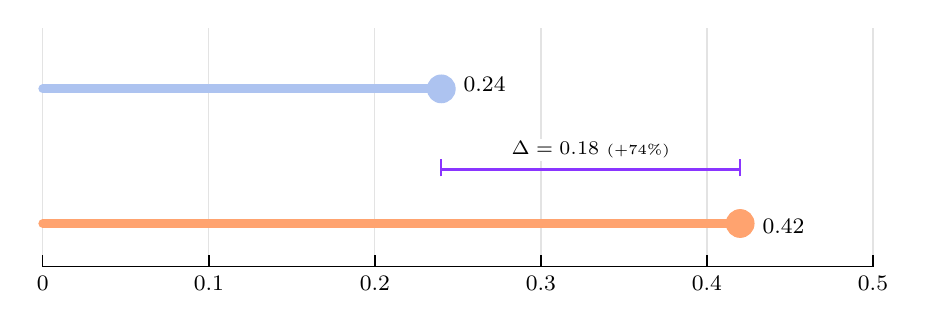
\begin{tikzpicture}
\begin{axis}[
  width=\columnwidth,
  height=0.38\columnwidth,
  xmin=0,
  xmax=0.5,
  ymin=-0.32,
  ymax=1.45,
  clip=false,
  axis x line*=bottom,
  axis y line=none,
  tick style={black, line width=0.5pt},
  xtick={0,0.1,0.2,0.3,0.4,0.5},
  xticklabels={0,0.1,0.2,0.3,0.4,0.5},
  xticklabel style={font=\footnotesize},
  ytick=\empty,
  xmajorgrids=true,
  major grid style={draw=gray!22, line width=0.45pt},
]

% High-control line
\addplot[
  highblue,
  line width=3.2pt,
  line cap=round
] coordinates {(0,1) (0.24,1)};

\addplot[
  only marks,
  mark=*,
  mark size=5.0pt,
  draw=highblue,
  fill=highblue
] coordinates {(0.24,1)};

% Low-control line
\addplot[
  loworange,
  line width=3.2pt,
  line cap=round
] coordinates {(0,0) (0.42,0)};

\addplot[
  only marks,
  mark=*,
  mark size=5.0pt,
  draw=loworange,
  fill=loworange
] coordinates {(0.42,0)};
% Value labels
\node[
  font=\footnotesize,
  anchor=west,
  fill=white,
  inner sep=0.7pt
] at (axis cs:0.252,1.03) {$0.24$};

\node[
  font=\footnotesize,
  anchor=west,
  fill=white,
  inner sep=0.7pt
] at (axis cs:0.432,-0.02) {$0.42$};

% Delta bracket
\draw[
  deltapurple,
  line width=0.85pt
] (axis cs:0.24,0.40) -- (axis cs:0.42,0.40);

\draw[
  deltapurple,
  line width=0.85pt
] (axis cs:0.24,0.35) -- (axis cs:0.24,0.48);

\draw[
  deltapurple,
  line width=0.85pt
] (axis cs:0.42,0.35) -- (axis cs:0.42,0.48);

\node[
  font=\scriptsize,
  anchor=south,
  fill=white,
  inner sep=1pt
] at (axis cs:0.33,0.46)
{$\Delta=0.18$ {\tiny$(+74\%)$}};

\end{axis}
\end{tikzpicture}
\caption{Mean cosine distance to the globally controlled reference ($\tau=10$) in the PartField feature space, comparing high-control (blue) and low-control (orange) regions over the assets of our test set.
\vspace{-4mm}}
\label{fig:control_regions_distance}
\end{figure}

\paragraph{Geometric and Textual Alignment.}
In addition to evaluating local feature-level variations, we assess the overall geometric precision and semantic alignment of our method using standard 3D generation metrics. Specifically, to measure spatial adherence to the input superquadrics, we compute the Chamfer Distance (CD) separately on the designated high-control ($CD_{\text{high}}$) and low-control ($CD_{\text{low}}$) regions. A lower $CD_{\text{high}}$ indicates closer compliance with the user's spatial constraints, whereas a higher $CD_{\text{low}}$ indicates that the model has the geometric freedom to reinterpret and detail the low-control regions. To evaluate semantic alignment, we compute the CLIP text distance between the rendered assets and the input prompts.

Table~\ref{tab:quantitative_spatial} presents the quantitative comparison between our local-$\tau$ method and two global baselines: $\tau = 3$ (weak global control) and $\tau = 10$ (strong global control). In the low-control regions, our method achieves a $CD_{\text{low}}$ of $11.39$, matching the flexibility of the weak baseline ($\tau = 3$). On the other hand, in the high-control regions, our method achieves a low error of $2.44$, closely approaching the strict compliance of the strong baseline ($\tau = 10$).

Furthermore, our CLIP text-alignment score ($0.243$) is comparable to both baselines. This demonstrates that introducing localized, variable control strengths does not degrade the prompt-following capabilities of the underlying model.

\begin{table}[t]
\centering
\small
\begin{tabular}{lccc}
\toprule
Method & $CD_{\text{high}} \downarrow$ & $CD_{\text{low}} \uparrow$ & CLIP-text $\downarrow$ \\
\midrule
$\tau=3$ & 9.29 $\pm$ 7.46 & 11.28 $\pm$ 13.95 & 0.247 $\pm$ 0.020 \\
local-$\tau$ & 2.44 $\pm$ 1.55 & 11.39 $\pm$ 17.32 & 0.243 $\pm$ 0.017 \\
$\tau=10$ & 0.87 $\pm$ 0.51 & 2.73 $\pm$ 5.51 & 0.235 $\pm$ 0.019 \\
\bottomrule
\end{tabular}
\caption{\textbf{Quantitative evaluation of spatial control and prompt alignment.} We report Chamfer Distance (CD) on high-control regions ($CD_{\text{high}} \downarrow$) and low-control regions ($CD_{\text{low}} \uparrow$), alongside CLIP text-image distance (CLIP-text $\downarrow$). Our local-$\tau$ control achieves strict geometric compliance in high-control areas (low $CD_{\text{high}}$) while matching the generative freedom of $\tau = 3$ in low-control areas (high $CD_{\text{low}}$), without compromising semantic alignment.}
\label{tab:quantitative_spatial}
\end{table}

\paragraph{User study.}
%In addition to geometric and feature space metrics, we conducted a pairwise user study for perceptual evaluation of the generated assets. Our local-$\tau$ control was compared against two global $\tau$ baselines, $\tau=3$ and $\tau=10$. For each of 19 test scenes we generated three outputs with local or global conditioning from the same superquadric inputs and prompts, and asked participants to compare local-$\tau$ against each baseline separately. Shown two outputs side by side as interactive 3D models, participants indicated which output followed the high- and low-control input superquadrics at the desired level of control, which looked more realistic and which they preferred overall. The study encompassed 39 individuals and 333 trials in total.

To complement our quantitative metrics, we conducted a pairwise user study evaluating the perceptual quality of the generated assets. We compared our local-$\tau$ control against uniform global baselines of $\tau = 3$ and $\tau = 10$. Using 19 test scenes, we generated three outputs (local-$\tau$, $\tau=3$, and $\tau=10$) from identical prompts and superquadric inputs. Participants viewed interactive 3D model pairs side-by-side and evaluated them based on shape fidelity, realism, and overall preference. The study collected 333 trials from 39 participants.

%Figure \ref{fig:user_study_local_tau} reports the resulting win/tie/loss rates. Against $\tau=3$, local-$\tau$ is preferred on shape fidelity in 81\% of comparisons, while remaining comparable on realism (47\% wins, 16\% ties) and overall preference (50\% wins, 15\% ties). Against $\tau=10$, local-$\tau$ is judged more realistic in 74\% of comparisons and preferred overall in 70\%. On shape fidelity, however, its win rate against $\tau=10$ drops to 37\%. We suspect this reflects how participants interpreted the question, which asked which object better matches the prompt in the low-control region while also following the input shape in the high-control region. Since $\tau=10$ follows the input shape closely everywhere, including the low-control region, participants may have judged overall resemblance to the input shape rather than distinguishing between the two regions. 

% Across both comparisons, local-$\tau$ conditioning avoids the trade-off that uniform control enforces on the entire object. Rather than fixing one global setting between fidelity and realism, it resolves that trade-off separately for each region of the asset. 


As shown in Fig.~\ref{fig:user_study_local_tau}, local-$\tau$ is preferred for shape fidelity in $81\%$ of comparisons against $\tau=3$, while achieving comparable results for realism ($47\%$ wins, $16\%$ ties) and overall preference ($50\%$ wins, $15\%$ ties). Against the higher control global baseline ($\tau=10$), local-$\tau$ is judged significantly more realistic ($74\%$ wins) and is preferred overall ($70\%$ wins). On shape fidelity, its win rate against $\tau=10$ falls to $37\%$. We attribute this to participants prioritizing overall resemblance to the input shape (which $\tau=10$ enforces globally) rather than evaluating only the high control region as requested. Overall, local-$\tau$ conditioning avoids the trade-off that uniform control enforces on the entire object. Rather than fixing one global setting between fidelity and realism, it resolves that trade-off separately for each region of the asset. 



%userstudy
% user study
\begin{figure}[t]
\centering
\resizebox{\columnwidth}{!}{%
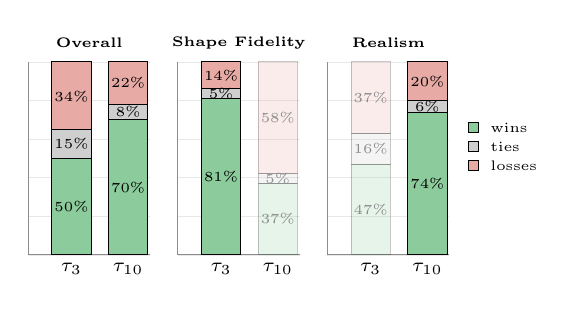
\begin{tikzpicture}

% ---------- colors ----------
\definecolor{wincol}{HTML}{8CCB9B}
\definecolor{tiecol}{HTML}{CFCFCF}
\definecolor{losscol}{HTML}{E7AAA5}

% ---------- dimensions ----------
\def\H{2.45}
\def\barw{0.5}
\def\xA{0.30}
\def\xB{1.02}
\def\panelw{1.55}

% ---------- panel macro ----------
\newcommand{\drawpanel}[3]{%
  % #1 = x offset, #2 = title, #3 = y labels? 1/0

  % grid
  \foreach \p in {0,20,40,60,80,100} {
    \pgfmathsetmacro{\yy}{\p*\H/100}
    \draw[gray!18, line width=0.25pt]
      ({#1},\yy) -- ({#1+\panelw},\yy);
  }

  % axes
  \draw[black!45, line width=0.35pt] ({#1},0) -- ({#1+\panelw},0);
  \draw[black!45, line width=0.35pt] ({#1},0) -- ({#1},\H);

  % y labels, no percent signs
  %\ifnum#3=1
    %\foreach \p in {0,20,40,60,80,100} {
     % \pgfmathsetmacro{\yy}{\p*\H/100}
     % \node[anchor=east, font=\tiny] at ({#1-0.04},\yy) {\p};
   % }
  %\fi

  % title
  \node[font=\bfseries\tiny, align=center]
    at ({#1+\panelw/2},{\H+0.24}) {#2};
}

% ---------- stacked bar macro ----------
\newcommand{\stackbar}[7]{%
  % #1 = x
  % #2 = wins
  % #3 = ties
  % #4 = losses
  % #5 = opacity
  % #6 = label color
  % #7 = show labels? 1/0

  \pgfmathsetmacro{\yw}{#2*\H/100}
  \pgfmathsetmacro{\yt}{#3*\H/100}
  \pgfmathsetmacro{\yl}{#4*\H/100}

  % wins
  \draw[
    fill=wincol,
    fill opacity=#5,
    draw=black,
    draw opacity=#5,
    line width=0.35pt
  ] (#1,0) rectangle ({#1+\barw},{\yw});

  % ties
  \draw[
    fill=tiecol,
    fill opacity=#5,
    draw=black,
    draw opacity=#5,
    line width=0.35pt
  ] (#1,\yw) rectangle ({#1+\barw},{\yw+\yt});

  % losses
  \draw[
    fill=losscol,
    fill opacity=#5,
    draw=black,
    draw opacity=#5,
    line width=0.35pt
  ] (#1,{\yw+\yt}) rectangle ({#1+\barw},\H);


  \ifnum#7=1
    \node[font=\tiny, text=#6]
      at ({#1+\barw/2},{\yw/2}) {#2\%};

    \node[font=\tiny, text=#6]
      at ({#1+\barw/2},{\yw+\yt/2}) {#3\%};

    \node[font=\tiny, text=#6]
      at ({#1+\barw/2},{\yw+\yt+\yl/2}) {#4\%};
  \fi
  

}

% ==================================================
% Overall
% ==================================================
\drawpanel{0}{Overall}{1}
\stackbar{0+\xA}{50}{15}{34}{1.0}{black}{1}
\stackbar{0+\xB}{70}{8}{22}{1.0}{black}{1}
\node[font=\scriptsize] at ({0+\xA+\barw/2},-0.18) {$\tau_{3}$};
\node[font=\scriptsize] at ({0+\xB+\barw/2},-0.18) {$\tau_{10}$};

% ==================================================
% Shape fidelity
% ==================================================
\drawpanel{1.90}{Shape Fidelity}{0}
\stackbar{1.90+\xA}{81}{5}{14}{1.0}{black}{1}
\stackbar{1.90+\xB}{37}{5}{58}{0.22}{black!45}{1}
\node[font=\scriptsize] at ({1.90+\xA+\barw/2},-0.18) {$\tau_{3}$};
\node[font=\scriptsize] at ({1.90+\xB+\barw/2},-0.18) {$\tau_{10}$};

% ==================================================
% Realism
% ==================================================
\drawpanel{3.80}{Realism}{0}
\stackbar{3.80+\xA}{47}{16}{37}{0.22}{black!45}{1}
\stackbar{3.80+\xB}{74}{6}{20}{1.0}{black}{1}
\node[font=\scriptsize] at ({3.80+\xA+\barw/2},-0.18) {$\tau_{3}$};
\node[font=\scriptsize] at ({3.80+\xB+\barw/2},-0.18) {$\tau_{10}$};

% ==================================================
% Compact legend
% ==================================================
\begin{scope}[shift={(5.72,1.55)}]
  \draw[fill=wincol, draw=black, line width=0.3pt] (-0.13,0.00) rectangle (0,0.13);
  \node[anchor=west, font=\tiny] at (0.03,0.065) {wins};

  \draw[fill=tiecol, draw=black, line width=0.3pt] (-0.13,-0.24) rectangle (0,-0.11);
  \node[anchor=west, font=\tiny] at (0.03,-0.175) {ties};

  \draw[fill=losscol, draw=black, line width=0.3pt] (-0.13,-0.48) rectangle (0,-0.35);
  \node[anchor=west, font=\tiny] at (0.03,-0.415) {losses};
\end{scope}

\end{tikzpicture}
}

\caption{User study comparing \methodname against fixed $\tau$ baselines. Dimmed bars show non-primary comparisons.}
\label{fig:user_study_local_tau}

\end{figure}


\subsection{Appearance Control}

\subsection{Joint Control}

\subsection{Ablations}
\input{sec/5_conclusions}

\newpage 

\ % The empty column

\newpage

\ % The empty column

\newpage

{
    \small
    \bibliographystyle{ieeenat_fullname}
    \bibliography{main}
}
\input{sec/X_suppl}

\end{document}
